% !TeX program = xelatex
\documentclass[11pt,a4paper]{article}
\usepackage[left=22mm,right=21mm,top=21mm,bottom=22mm,footskip=11mm]{geometry}
\usepackage{fontspec}
\setmainfont{DejaVu Serif}
\setsansfont{DejaVu Sans}
\setmonofont{DejaVu Sans Mono}[Scale=0.87]
\usepackage[english,russian]{babel}
\usepackage{amsmath,unicode-math,graphicx,array,booktabs,tabularx,enumitem,caption,titlesec,fancyhdr,catchfile}
\CatchFileDef{\rowsA}{tables/a.tex}{\endlinechar=-1 }
\CatchFileDef{\rowsB}{tables/b.tex}{\endlinechar=-1 }
\usepackage[unicode,hidelinks]{hyperref}
\hypersetup{pdftitle={Экспериментальное сравнение сканеров},pdfauthor={Гуцалов Егор Никитич, Лемдянов Илья Данилович},pdflang={ru}}
\captionsetup{font=small,labelfont=bf,labelsep=period,justification=raggedright,singlelinecheck=false,hypcap=false}
\addto\captionsrussian{\renewcommand{\figurename}{Рис.}\renewcommand{\tablename}{Таблица}}
\titleformat{\section}{\sffamily\bfseries\LARGE}{\thesection.}{.4em}{}
\titlespacing*{\section}{0pt}{0pt}{12pt}
\newcommand{\subhead}[1]{\par\addvspace{8pt}\noindent\textbf{#1}\par\nobreak}
\newcommand{\code}[1]{\texttt{#1}}
\newcommand{\timecell}[3]{\shortstack{#1\\[.3pt]{\fontsize{8.1}{9}\selectfont [#2; #3]}}}
\newcommand{\sourcega}[2]{\cite[п.~#1, слайд~#2]{ga}}
\newcommand{\nextpage}{\clearpage}
\setlength{\parindent}{1.35em}
\setlength{\parskip}{3.6pt plus .4pt minus .3pt}
\setlength{\emergencystretch}{1.5em}
\setlist[enumerate]{leftmargin=2em,itemsep=5pt,topsep=4pt,parsep=0pt}
\setlength{\headheight}{14pt}
\pagestyle{fancy}\fancyhf{}
\fancyfoot[L]{\footnotesize\sffamily Экспериментальное сравнение сканеров}
\fancyfoot[R]{\small\sffamily\thepage}
\renewcommand{\headrulewidth}{0pt}
\renewcommand{\footrulewidth}{0.3pt}
\raggedbottom
\begin{document}
\begin{titlepage}
\thispagestyle{empty}
\centering
{\large Санкт-Петербургский политехнический университет\\[3pt] Петра Великого\par}
\vspace{30mm}
{\sffamily\bfseries\fontsize{31}{37}\selectfont Экспериментальное\\сравнение сканеров\par}
\vspace{8mm}
{\Large Как время лексического анализа зависит\\[3pt] от реализации сканера и свойств текста?\par}
\vspace{13mm}
{\normalsize Обзорный научно-популярный доклад\\
Самостоятельная научно-исследовательская работа студента (СНИРС)\\
по теме к разделу 2.6 курса «Грамматики и автоматы»\par}
\vfill
{\large Гуцалов Егор Никитич\\[3pt] Лемдянов Илья Данилович\par}
\vspace{3mm}
Группа 5030102/30201\par
\vspace{18mm}
Санкт-Петербург, 2026
\end{titlepage}
\setcounter{page}{2}

\section*{Коротко о главном}
Слово \code{if} обозначает условие, а \code{if2} может быть именем переменной. Сканер обязан различать их при любом устройстве программы. Мы задали четырём сканерам одни правила, проверили выдачу по каждому байтовому интервалу и измерили полный проход по 21 тексту. За единицу сравнения взяли время прохода, делённое на число байтов входа.

\begin{enumerate}
\item \textbf{На учебном псевдокоде быстрее всего оказался re2c.}
Его медиана составила 2,478~нс/байт. Ближайший результат у собственного варианта с ветвлениями, 3,432~нс/байт. На смеси из повторений строки с условным оператором наименьшее время при всех трёх объёмах показал табличный сканер.
\item \textbf{Длина лексемы меняет результат даже при одинаковом объёме файла.}
На идентификаторах из двух букв таблица выигрывала у ветвлений во всех 16 раундах. На идентификаторах из 32 и 128 букв во всех раундах выигрывали ветвления. Для длины 128 медиана парного отношения времён достигла 3,245.
\item \textbf{Близкие результаты требуют оговорки.} На повторениях \code{abcde2} медианы \code{table} и \code{re2c} равны 1,551 и 1,555~нс/байт. Межквартильные интервалы перекрываются. На этом входе данные не дают основания предпочесть одну из этих программ по скорости.
\end{enumerate}
В конце даны три рекомендации по выбору и сравнению сканеров.

\subhead{Что получает сканер}
Первая строка корпуса взята из записи функции модуля числа:
\begin{center}
\code{abs(x) := if x>0 then x else -x end if}
\end{center}
Сканер выдаёт вид и границы каждой лексемы. Получатель может отличить имя \code{abs} от ключевого слова \code{if}, найти присваивание и извлечь исходное написание числа. Для этой задачи не требуется проверять синтаксис условного оператора или вычислять значение функции \sourcega{3.2.1}{1/4}.

\begin{center}
\captionof{table}{Лексика выбранного псевдокода. В первых двух строках приведены регулярные выражения, в остальных~--- полный перечень написаний.}
\small\renewcommand{\arraystretch}{1.18}
\begin{tabularx}{\linewidth}{@{}lX@{}}\toprule
Идентификатор & \code{[A-Za-z][A-Za-z0-9]*}\\
Десятичное число & \code{[0-9]+}\\
Ключевые слова & \code{if then else end while do for from to return case}\\
Знаки и разделители & \code{:= \ = \ != \ < \ <= \ > \ >= \ + \ - \ * \ / \ ( \ ) \ [ \ ] \ , \ ; \ :}\\ \bottomrule
\end{tabularx}
\end{center}

\nextpage
\section{Одна лексика, четыре реализации}
Учебный псевдокод допускает математическую запись \sourcega{0.2.4}{1/5}. Для опыта мы зафиксировали её байтовое представление. Идентификатор начинается с латинской буквы и продолжается буквами или цифрами. Число состоит из одной или нескольких десятичных цифр. Это два класса слов, задаваемых регулярными выражениями \cite[п.~1.2.1, слайды 1/3--2/3]{ga}. Ещё 11 видов отведены ключевым словам и 18~--- знакам и разделителям. Всего сканер различает 31 обычный вид лексемы.

В каждой позиции выбирается самое длинное подходящее слово. При равной длине ключевое слово имеет приоритет над идентификатором. Пробел, табуляция, возврат каретки и перевод строки пропускаются. Комментарий \code{//} продолжается до конца строки или входа. При ошибке в позиции $p$ сканер выдаёт интервал $[p,p+1)$, в конце текста длины $N$~--- признак конца файла (EOF, от английского \textnormal{end of file}) с интервалом $[N,N)$. Позиции нумеруются с нуля. В правую границу интервала байт уже не входит.

Для каждого вида лексемы нужны состояния, в которых прочитанное слово можно принять. В модели автомата-распознавателя это заключительные состояния \sourcega{2.2.1}{1/2}. Сканер дополнительно хранит вид принятого слова и его правую границу.

\begin{center}
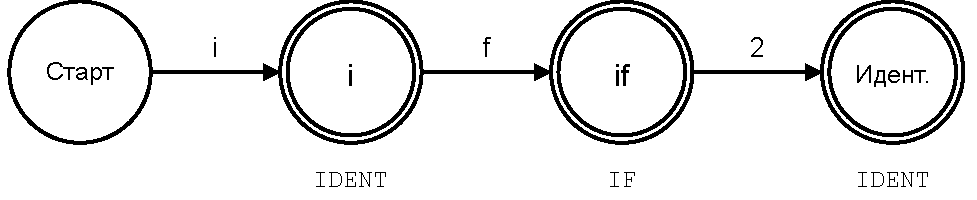
\includegraphics[width=.85\linewidth]{figures/prefix.pdf}
\captionof{figure}{Путь детерминированного конечного автомата (ДКА) по слову \code{if2}. Стрелка подписана прочитанным байтом. Двойной круг обозначает заключительное состояние. Под ним указан вид лексемы при остановке в этой позиции. На рисунке показаны только переходы данного пути.}\label{fig:path}
\end{center}

После двух байтов автомат запоминает \code{IF} и конец слова в позиции~2. Третий байт допускает продолжение и меняет запомненную пару на \code{IDENT} и~3. По окончании входа выдаётся один идентификатор $[0,3)$. В записи \code{if:=15} двоеточие завершает поиск первого слова. Получаются \code{IF} $[0,2)$, присваивание $[2,4)$ и число $[4,6)$.

\textbf{flex} получает правила и строит программу на C с полной таблицей переходов (ключ \code{-Cf}) \cite{flex}. \textbf{re2c} по правилам строит программу на C с проверками байта и переходами к меткам \cite{re2c}. У двух собственных сканеров на C++ один шаблон выделения лексем. В \textbf{table} переход получается чтением элемента массива, в \textbf{branch} его задают ветвления по состоянию и классу байта. Учебник сопоставляет эти способы в пп.~2.6.1 и 2.6.2 \cite[п.~2.6.1, слайды 1/3--2/3; п.~2.6.2, слайды 1/3 и 3/3]{ga}.

\nextpage
\section{Как проводились измерения}
Для каждого входа независимая программа на Python заранее выписала ожидаемые тройки «вид, начало, конец». До прогрева стенд сравнил с ними каждую тройку всех четырёх сканеров, включая EOF. После EOF проверен повторный вызов. Отдельные тесты охватили все 31 вида, пустой текст, ошибочный байт, комментарий без перевода строки и лексему у конца буфера.

\subhead{Что означает наносекунда на байт}
Пусть $N$~--- число байтов в файле, включая пробелы, комментарии и переводы строк. $K$~--- число выданных обычных лексем, без EOF. Перед запуском файл уже находился в памяти и экземпляры сканера были открыты. Счётчик времени включали перед первым \code{next}. В интервал вошли вызовы до EOF включительно, подсчёт лексем и одинаковое для четырёх вариантов обновление 64-битной контрольной суммы по виду и обеим границам. Закрытие экземпляров, сверку с эталоном и запись результата выполняли после остановки счётчика.

Пусть $E$~--- длительность измеренного интервала в наносекундах, $P$~--- число полных проходов в нём. При $N<65\,536$ выполняли $P=16$ проходов, иначе $P=1$. Время одного прохода $T=E/P$. В таблицы вошёл показатель
\[
             t=\frac{T}{N}=\frac{E}{P\,N}\quad\text{нс/байт}.
\]
Например, для корпуса $P\,N=16\cdot17\,430=278\,880$ байт. Так учитываются и байты, которые сканер прочитал и пропустил. Показатель характеризует полную обработку входа вместе с выдачей результата.

\begin{center}\captionof{table}{Условия общей серии А и Б.}\label{tab:env}
\small\begin{tabularx}{\linewidth}{@{}lX@{}}\toprule
Процессор и система & Intel Core i5-13400F, Windows 11 25H2, сборка 26200\\
Компиляция & Компиляторы \code{gcc} и \code{g++} 13.2.0 из MinGW-w64. Параметры оптимизации \code{-O3 -DNDEBUG}. Стенд и сгенерированные сканеры написаны на C11, собственный сканер~--- на C++17.\\
Генераторы и часы & win\_flex 2.6.4 (\code{-8 -Cf}), re2c 4.6. Время измерено системным счётчиком \code{QueryPerformanceCounter}.\\
Порядок & Один прогрев на вариант и вход, затем 16 раундов. Первый порядок: flex, re2c, table, branch. В каждом следующем раунде первый вариант перемещался в конец.\\ \bottomrule
\end{tabularx}\end{center}
Для каждого входа и варианта указаны медиана и квартили $Q_1$, $Q_3$ по 16 раундам. Для доли $p$ берётся позиция $15p$ в отсортированном ряду с нумерацией от нуля и линейной интерполяцией. Интервал между квартилями описывает среднюю половину замеров.

\nextpage
\section{Что менялось во входном тексте}
\subhead{Учебный корпус}
Из псевдокода курса подготовлены 72 фрагмента. Первый содержит функцию модуля, далее встречаются преобразования грамматик, обходы и проверки условий. Для записи в текстовый файл знак присваивания приведён к \code{:=}, знак «меньше или равно» к \code{<=}, а греческие буквы в именах заменены словами, например \code{alpha}. Список замен приложен к исходникам. Замерялся один и тот же файл без преобразования переводов строк. Его объём 17\,430 байт, в том числе 530 двухбайтовых переводов строки. На пропуски приходится 46,6\,\% байтов. Среди 3\,792 выданных лексем есть все 31 вида, в том числе 1\,750 идентификаторов и 137 чисел.

\subhead{Общие начала слов}
В трёх файлах по 1\,048\,576 байт повторяются \code{abx}, чередующиеся \code{abx} и \code{ifx} или только \code{ifx}. Далее сравниваются слова длины шесть \code{abcde2} и \code{while2}. За каждым словом стоит один пробел. Внутри каждой группы совпадают объём, число, виды и границы лексем. Меняется доля слов, у которых автомат сначала проходит по началу ключевого слова. Несмотря на это, результатом всякий раз служит один идентификатор.

\subhead{Длина идентификатора и числа}
В файл объёмом $2^{20}$ байт помещаются блоки из 2, 8, 32 или 128 букв \code{a} и одного пробела. Остаток в конце заполняется пробелами. Процедуру повторяют с цифрой \code{1}. Меняются длина лексемы и число выдач за проход. Доля пробелов тоже меняется. Пара «буквы~--- цифры» одной длины даёт одинаковые размеры и позиции лексем при разных видах.

\subhead{Пробелы и комментарии}
Первый файл содержит строки из \code{x}, семи пробелов и перевода строки. Во втором через строку семь пробелов заменены на \code{//aaaaa}, в третьем заменены все. Границы всех \code{x} совпадают. В четвёртом файле на каждые 64 имени приходится один длинный комментарий. Как и в третьем файле, на комментарии приходится 448 байт на 64 имени. Теперь позиции отдельных имён изменились. Во всех четырёх случаях $N=1\,179\,648$, $K=131\,072$.

\subhead{Объём при постоянном составе}
Строка \code{if x:=15 then return x end if} вместе с переводом строки занимает 30 байт и даёт 9 лексем. Её повторяют 2\,048, 32\,768 и 524\,288 раз. Каждый шаг увеличивает $N$ и $K$ в 16 раз, а число выдач на один входной байт остаётся равным $9/30$.

\nextpage
\section{Опыт А. Четыре сканера}
Какой сканер быстрее на учебном корпусе и сохранится ли его преимущество при замене текста? В первом опыте время включает весь путь от чтения очередного байта до выдачи и учёта лексемы. Каждый столбец таблицы~\ref{tab:a} получен из одной и той же серии раундов.

\begin{center}
\captionof{table}{Время четырёх сканеров в нс/байт. В каждой ячейке сверху дана медиана, снизу~--- $[Q_1;Q_3]$. $N$ измеряется в байтах, $K$~--- число лексем без EOF.}\label{tab:a}
\setlength{\tabcolsep}{2pt}
\fontsize{9.1}{10.5}\selectfont
\begin{tabular*}{\linewidth}{@{\extracolsep{\fill}}lrrcccc@{}}
\toprule Вход & $N$ & $K$ & flex & re2c & table & branch\\ \midrule
\rowsA
\bottomrule
\end{tabular*}
\end{center}
На корпусе первым оказался re2c. Даже его верхний квартиль (2,561~нс/байт) ниже нижнего квартиля ближайшего варианта branch (3,386~нс/байт). На двухбайтовых именах и числах, а также на всех трёх размерах смешанного текста наименьшее время показала таблица.

\nextpage
\section*{Когда меняется самый быстрый сканер}
При фиксированном объёме одна переменная особенно заметно меняет результат: сколько байтов успевает прочитать сканер до очередной выдачи лексемы. На рис.~\ref{fig:length} для каждой длины взяты данные из двух строк таблицы~\ref{tab:a}, одной с буквами и одной с цифрами.

\begin{center}
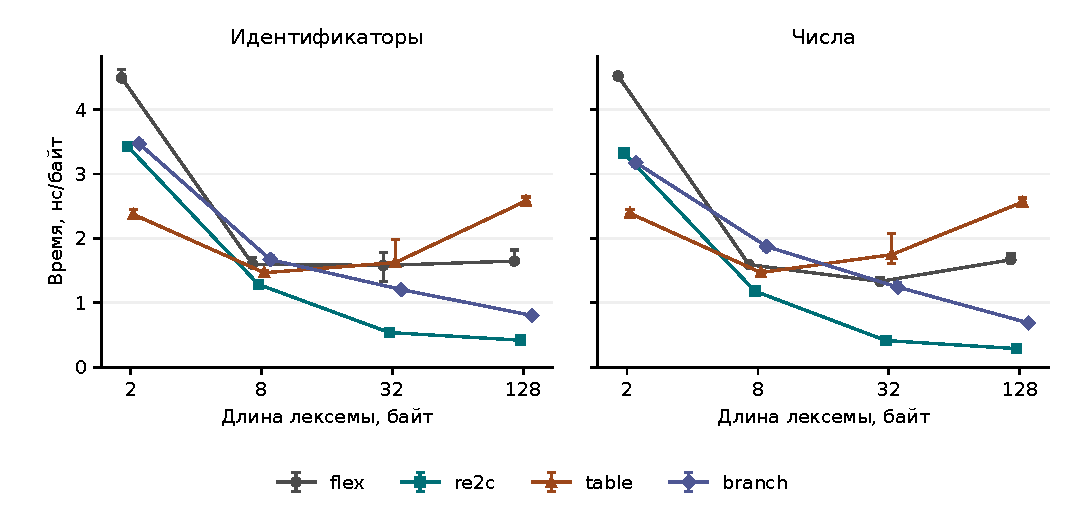
\includegraphics[width=\linewidth]{figures/length.pdf}
\captionof{figure}{Медиана времени полного прохода на байт при объёме $2^{20}$ байт. Маркеры различают четыре реализации, вертикальные отрезки показывают $[Q_1;Q_3]$. Горизонтальная ось логарифмическая по основанию 4, значения подписаны в байтах. Маркеры немного разведены по горизонтали для чтения интервалов.}\label{fig:length}
\end{center}

\subhead{Короткое слово и длинное слово}
При длине~2 наименьшая медиана у table в обеих сериях, а начиная с проверенной длины~8~--- у re2c. У последнего на числах она падает с 3,322 до 0,288~нс/байт. На идентификаторах той же длины~--- с 3,429 до 0,419. При этом $K$ уменьшается с 349\,525 до 8\,128. Время учёта одной выдачи распределяется на большее число байтов. Одного этого объяснения недостаточно: у table время на байт при переходе с 32 до 128 букв, наоборот, возрастает.

\subhead{Повторение одного и того же оператора}
На младшем, среднем и старшем объёмах у table получено 2,161, 2,159 и 2,197~нс/байт. Их межквартильные интервалы перекрываются. Объём самого большого файла в 256 раз больше первого. Полное время прохода возрастает примерно с 0,133 до 34,56~мс. Для этой периодической смеси переход к большому файлу мало изменил расходы на байт. Три размера не определяют закон роста для произвольного текста.

\subhead{Пограничные случаи}
По минимуму медианы re2c оказался первым на 11 входах, table~--- на 10. На \code{abcde2} медианы этих программ отличаются на 0,004~нс/байт. На длинных комментариях у re2c и branch получены 1,388 и 1,397~нс/байт. На первом входе table опередил re2c в 10 раундах из 16, на втором re2c опередил branch в 9 из 16. У каждой пары разница медиан мала на фоне разброса.

\nextpage
\section{Опыт Б. Два представления переходов}
У собственных вариантов общий граф и один шаблон \code{next}. Одно и то же число $c(a)$ обозначает класс входного байта $a$. В варианте table новое состояние равно элементу $D[q,c(a)]$, в branch~--- значению, которое выбирает вложенное ветвление по $q$ и $c(a)$. Генератор построил обе записи из одного описания. Тест перебрал 61 состояние и все 256 значений байта. Для всех $61\cdot256=15\,616$ пар значения совпали. Следовательно, одинаковое начальное состояние даёт одинаковый путь по любому слову. Метки заключительных состояний и правило выдачи тоже общие.

Классификатор объединяет байты с одинаковыми переходами из всех состояний в 36 классов и занимает 256 байт. Для table массив переходов занимает ещё $61\cdot36=2\,196$ байт. В branch этот шаг выражен операторами \code{switch}. Независимый процедурный сканер подтвердил выдачу собственных вариантов на 81\,685 проверочных входах.

Для каждого входа и раунда $r$ взяты два времени из опыта~А:
\[
            R_r=T_{\mathrm{table},r}/T_{\mathrm{branch},r}.
\]
При $R_r>1$ быстрее branch, при $R_r<1$ быстрее table. Квартили вычислены после образования 16 пар.

\begin{center}
\captionof{table}{Парное отношение времён на тех же входах, что в таблице~\ref{tab:a}. Последний столбец показывает число раундов из 16, в которых быстрее branch. Значения $R$ безразмерны.}\label{tab:b}
\small\setlength{\tabcolsep}{5pt}\renewcommand{\arraystretch}{1.04}
\begin{tabular*}{.95\linewidth}{@{\extracolsep{\fill}}lrrrr@{}}
\toprule Вход & Медиана $R$ & $Q_1$ & $Q_3$ & Побед branch\\ \midrule
\rowsB
\bottomrule
\end{tabular*}
\end{center}

\nextpage
\section*{Где выгодны таблица и ветвления}
На учебном корпусе медиана $R$ равна 1,046, а средняя половина парных отношений лежит между 1,023 и 1,066. В 13 из 16 раундов branch закончил проход раньше. Направление большинства пар видно и при частичном перекрытии интервалов отдельных реализаций в опыте~А. Выигрыш на корпусе скромнее, чем на длинных однородных словах.

\begin{center}
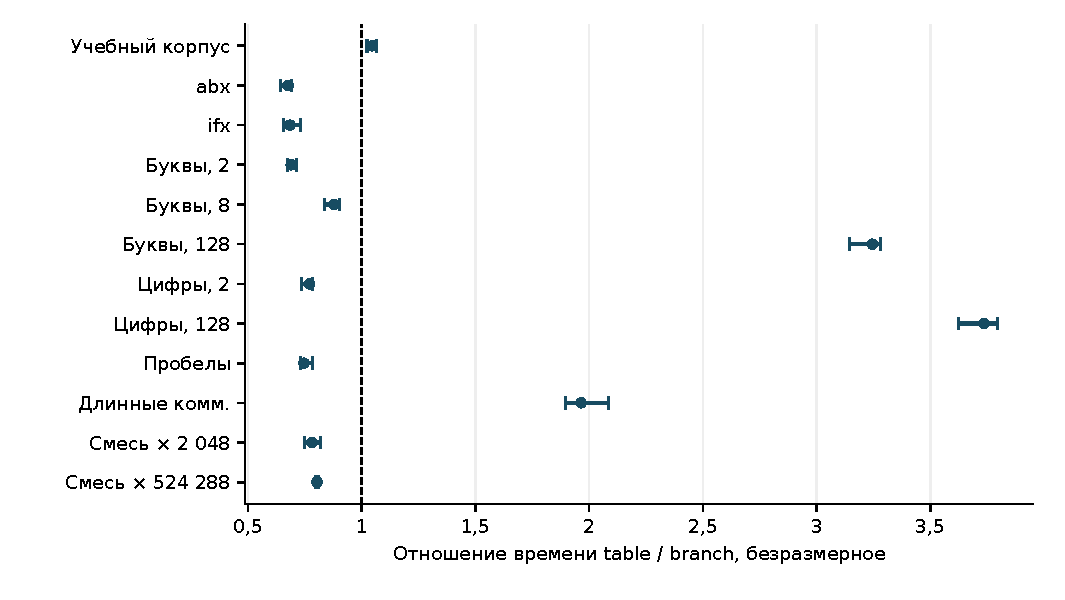
\includegraphics[width=.96\linewidth]{figures/ratios.pdf}
\captionof{figure}{Выбранные входы из таблицы~\ref{tab:b}. Точка~--- медиана парных отношений, горизонтальный отрезок~--- $[Q_1;Q_3]$. Штриховая вертикаль соответствует равному времени. Слева быстрее table, справа быстрее branch.}\label{fig:ratios}
\end{center}

\subhead{Что даёт общее начало с ключевым словом}
При замене всех \code{abx} на \code{ifx} медиана $R$ меняется с 0,677 до 0,685. Как и на смеси этих слов, во всех 16 парах выигрывает table. Для шестибайтовых слов переход от \code{abcde2} к \code{while2} приближает отношение к единице (с 0,803 до 0,932). Длина и выдача сохранены, но слово \code{while2} проводит автомат через состояния префикса ключевого слова. Влияние этого изменения зависит от выбранной пары.

\subhead{Одинаковое число имён, разное устройство пропусков}
На коротких комментариях $R=0,779$, на длинных $R=1,965$. В обоих случаях одинаковы объём входа, число имён и суммарный размер комментариев. В первом случае сканер часто входит в состояние комментария и покидает его. Во втором он дольше остаётся в этом состоянии. Направление преимущества изменилось во всех 16 парах. Чтобы отделить влияние ветвлений процессора от обращений к памяти, понадобились бы отдельные измерения.

\nextpage
\section*{Выводы и рекомендации}
На учебном корпусе для готового сканера re2c получено 2,478~нс/байт. В контролируемом сравнении двух представлений одного автомата на том же корпусе branch имеет меньшую медиану, а превосходство table на трёх размерах смешанной строки сохраняется в каждом раунде. Следовательно, ответ на вопрос о скорости зависит и от реализации, и от того, какими путями текст проводит автомат между выдачами лексем.

\begin{enumerate}
\item \textbf{Для обработки учебного псевдокода начать с re2c.}
На данном корпусе его межквартильный интервал отделён от интервалов остальных трёх сканеров. Если вход в основном состоит из коротких имён, стоит отдельно измерить табличный вариант: на двухбуквенных именах он вышел на первое место.
\item \textbf{При выборе представления собственного автомата учитывать длину слов и пропусков.}
На именах из 2 и 8 букв выигрывала таблица, на именах из 32 и 128 букв~--- ветвления. Аналогичная смена обнаружена при укрупнении комментариев с сохранением их общего объёма. Число состояний автомата во всех запусках одинаково.
\item \textbf{Близкие варианты сравнивать по общим раундам и указывать разброс.}
На \code{abcde2} и на длинных комментариях два первых результата опыта~А практически совпали. Для собственной пары на учебном корпусе в трёх раундах из 16 порядок также оказался обратным большинству. Для выбора на другой машине требуется повторение серии.
\end{enumerate}

\subhead{Ограничения}
Все выводы относятся к одной машине, одной оптимизированной сборке, одному учебному корпусу и четырём семействам искусственных текстов. Перед замером проводился прогрев. Привязку к ядру и частоту процессора не фиксировали. Учитывались выдача лексем и контрольная сумма. Подготовка буферов, чтение с диска и время построения сканеров в оценку не входят. Аппаратные счётчики обращений к памяти и ошибок предсказания переходов не снимались. Межквартильный размах характеризует эту серию из 16 раундов.

\begingroup\small
\renewcommand{\refname}{Источники}
\begin{thebibliography}{9}\setlength{\itemsep}{2pt}\setlength{\parskip}{0pt}
\bibitem{ga} Новиков Ф.~А. Грамматики и автоматы. Материалы курса. СПб., 2026. Пп.~0.2.4, 1.2.1, 2.2.1, 2.6.1, 2.6.2, 3.2.1. Для слайдов в тексте приведены их номера внутри пункта.
\bibitem{flex} The flex project. Lexical Analysis With Flex. Разделы \href{https://westes.github.io/flex/manual/Matching.html}{«How the Input Is Matched»} и \href{https://westes.github.io/flex/manual/Options-for-Scanner-Speed-and-Size.html}{«Options for Scanner Speed and Size»} (ключ \code{-Cf}). \url{https://westes.github.io/flex/manual/}. Дата обращения 28.11.2026.
\bibitem{re2c} The re2c project. User manual (C/C++). Раздел «Options», параметр \code{-{}-code-model}, модель \code{goto-label}. \url{https://re2c.org/manual/manual_c.html}. Дата обращения 28.11.2026.
\end{thebibliography}
\endgroup

\end{document}
